\chapter{Introduction}\label{ch:introduction}
\graphicspath{{../Figures/10-introduction/}{figs/10-introduction/}}

\section{Motivation}

Biomimetic robots provide a platform for investigating how mechanical structure and control interact to generate movement, offering complementary insights to simulation-based studies \citep{andrews_general_1985, millard_flexing_2013, arnold_model_2010}. Wheeled robots remain the platform of choice in structured environments, where their speed, efficiency, and payload capacity are difficult to match; in the unstructured terrain of the natural and built world, legged machines hold the advantage, and biomimetic legs that reproduce human force capabilities have the potential to excel where wheels cannot \citep{frey_legged_2026, ha_learning_2025}. Musculoskeletal humanoids and limb systems driven by tendon-like actuators have been shown to support biologically meaningful experiments on motion generation, internal force transmission, and neural control hypotheses \citep{asano_design_2017, asano_musculoskeletal_2019, hitzmann_anthropomorphic_2018, liu_robotic_2018, chen_realizing_2019}. The dual perspective of using robots to learn about biology, and using biology to design more adaptive robots, has been emphasized in both biomimetic robotics and biomechanics \citep{ijspeert_amphibious_2020, asano_design_2017}. With such robotic systems, experiments can be performed that would not be practical or ethical with human test subjects, such as removing a specific muscle from the system or blocking a sensory feedback pathway. Experiments of this kind allow direct testing of how the components of the neuromechanical system interact, and they offer new opportunities for testing neural control theories that are faster and cheaper than human observation studies \citep{shin_constructive_2018, goldsmith_investigating_2021, schilling_adaptive_2022}.

Artificial muscles are a key enabling technology for this class of robot. Among the available actuation technologies, McKibben-style braided pneumatic actuators (BPAs) combine low mass, high force-to-weight ratio, and intrinsic compliance with a force--length curve that qualitatively resembles that of skeletal muscle \citep{liang_comparative_2020, hunt_modeling_2017}. BPAs have been used in quadrupedal robots \citep{aschenbeck_design_2006, hunt_modeling_2017, scharzenberger_design_2019}, musculoskeletal humanoids \citep{asano_design_2017, hitzmann_anthropomorphic_2018}, and dexterous manipulation systems \citep{chen_realizing_2019}. However, BPAs also differ from biological muscle in important ways: their maximum tensile force occurs at resting length rather than at an optimal fiber length, their maximum contraction ratio is substantially lower than that of human muscle, and their force output is a highly nonlinear function of internal pressure, contraction, and loading state \citep{hunt_modeling_2017, sarosi_comparative_2017, liang_comparative_2020}. The author's experience with \qty{10}{\mm} actuators made this gap concrete: manufacturer specifications overstate the force and contraction available at the short resting lengths a leg design requires, and designs based on those specifications delivered less range of motion and joint torque than intended. Nor could the published empirical models repair the discrepancy, because each is fitted to measurements at a single resting length \citep{sarosi_comparative_2017, martens_modeling_2017, hunt_modeling_2017}; none accurately predicts how force changes when a designer chooses a different actuator length. Because muscle resting length is one of the primary degrees of freedom available to the robot designer, the absence of a force model valid at arbitrary resting length blocked rational actuator selection. Designing a biomimetic robot around BPAs therefore requires quantitative, predictive models of the actuator and of the joint torques it can produce.

Actuator force alone, however, does not determine the torque a joint produces. The robot knee transmits BPA force to the skeleton through mounting brackets, artificial tendons, and paths that wrap over the joint, and each of these elements departs from the rigid-body idealization: brackets and fixtures deflect under load, tendons stretch, and a wrapping actuator loses usable length as the knee flexes. At the start of this work it was unknown how much these transmission effects reduce the torque delivered at the knee relative to the rigid-body prediction, and no method existed for correcting that prediction in a form that would transfer between joint configurations. The biomimetic knee's optimized muscle routing \citep{morrow_optimization_2020} compounded the problem: it had never been validated experimentally or compared against human isometric torque data, so even the nominal torque envelope of the robot leg rested on unverified calculations.

There are additional gaps concerning the development of more detailed neural control models of locomotion and balance. One lies in the literature itself: the physiological properties of the group Ia, group Ib, and group II afferents that should inform the feedback design are scattered across a primary literature that the database of Chapter~\ref{ch:database} alone audits at 943 papers and reviews \citep{van_de_crommert_review_1998, windhorst_muscle_2007, windhorst_spinal_2022}, with no structured resource from which a robot designer or an animal researcher could draw them. The other lies in methods: no simulation pipeline existed for closing the loop between a musculoskeletal robot model of this kind and a biologically grounded neural controller. The neuromechanical modeling literature provides the ingredients, including two-level spinal central pattern generator architectures \citep{rybak_modelling_2006, mccrea_organization_2008}, neuromechanical simulation frameworks \citep{markin_afferent_2010}, and synthetic nervous system design tools \citep{nourse_sns_2023}, but it does not provide their assembly for a BPA-driven bipedal robot with human-like muscle routing: the conversion of the robot's own model into a simulation engine, the wiring of the rhythm and reflex circuits with their afferent feedback, and the closed-loop coupling of controller and mechanics in one runnable environment.

Four gaps thus stood between the existing robot design methods and a robot that can walk under neural control, in the order the chapters of this dissertation address them: no actuator force model valid at arbitrary resting length, no quantified correction for the torque lost through brackets, tendons, and wrapping, no consolidated resource for the afferent data that such a controller requires, and no closed-loop simulation pipeline joining the robot's musculoskeletal model to a biologically grounded neural controller.

\section{The Biomimetic Humanoid Robot Project}\label{sec:project}

This dissertation is part of a long-running effort at Portland State University to build a biomimetic humanoid robot from the trunk down, actuated by pneumatic artificial muscles and controlled by a synthetic nervous system (SNS). The project is deliberately iterative. Knowledge from biomechanics and neuroscience guides the design of robots intended to perform complex tasks in unstructured environments with improved efficiency, balance, adaptability, and resilience. Those robots then become physical models with which biological hypotheses can be tested, validated, and refined through controlled changes that would be impractical or unethical in living subjects. The resulting biological insight informs the next generation of robot design, and lessons from both directions can be translated into improved prosthetic and orthotic devices.

The present work builds directly on a series of studies by me and my collaborators. In my master's project, the kinematics and dynamics of a biomimetic robot leg were matched against the Gait2392 OpenSim model, artificial muscle attachment and wrapping locations were determined for the robot legs, and MATLAB tooling was developed for evaluating muscle lengths, moment arms, and isometric joint torques over the full range of motion \citep{bolen_bipedal_2019, bolen_determination_2019}. That work showed that simply transplanting human muscle attachment locations onto a BPA-actuated robot does not reproduce human torque profiles; the placement optimization that closes this gap was completed during this dissertation and is summarized in Section~\ref{sec:foundation}. The rest of the platform advanced in parallel, and this dissertation builds on its hardware and demonstrations: the biomimetic four-bar knee linkage with a migrating instantaneous center of rotation, designed and validated by Steele \citep{steele_development_2017, steele_biomimetic_2018, steele_biomimetic_2018-1}, is the knee of the robot leg whose torque transmission Chapter~\ref{ch:torque} measures, and the canine-inspired quadruped platform Muscle Mutt, formerly called DoggyDeux, demonstrated antagonistic BPA pairs under synthetic nervous system control on a physical robot \citep{scharzenberger_design_2019}, extending an earlier AARL demonstration of central pattern generator control of a pneumatically actuated robot \citep{hunt_development_2017}. The humanoid leg of this dissertation carries that line forward.

\section{Research Objectives}\label{sec:objectives}

This dissertation addresses the actuator-force and torque-correction gaps experimentally, resolves the afferent-data gap by consolidating the afferent literature into the Sensory Afferent Database \citep{bolen_sensory_2023, bolen_using_2024}, and closes the simulation-pipeline gap with the tools and framework of the final research chapter. The objectives are:

\begin{enumerate}
    \item \textbf{Characterize the isometric force of Festo BPAs} with uninflated diameters of \qtylist{10;20}{\mm} over a wide range of resting lengths, contractions, and pressures; derive improved maximum-force and normalized force--strain--pressure models; and compare them against existing models (Chapter~\ref{ch:muscles}).
    \item \textbf{Validate and improve the prediction of isometric knee torque} produced by BPAs on pinned-joint and biomimetic four-bar knees; identify and model losses caused by constant length offsets, series compliance, and actuator wrapping; and compare the resulting torque envelopes with human capabilities (Chapter~\ref{ch:torque}).
    \item \textbf{Consolidate the sensory afferent literature into a structured afferent resource}, the Sensory Afferent Database, by auditing and curating the published record of afferent properties across animal species and their role in motor control, and by evaluating AI-assisted literature triage for expanding the corpus (Chapter~\ref{ch:database}).
    \item \textbf{Develop tools and a framework for neuromechanical control} of the humanoid robot by converting its OpenSim musculoskeletal model to MuJoCo, implementing an SNS-Toolbox two-level spinal CPG with proprioceptive and heel/toe contact feedback, and establishing a staged tuning and verification workflow (Chapters~\ref{ch:sns} and~\ref{ch:overall}).
\end{enumerate}

\section{Dissertation Organization}\label{sec:organization}

Chapter~\ref{ch:background} establishes the technical and scientific context for the dissertation. It reviews biomimetic and musculoskeletal robots, robot actuation technologies with an emphasis on braided pneumatic actuators and published models of their force--length--pressure behavior, and the human lower-limb biomechanics and OpenSim benchmark models that serve as design targets. It then covers the computational neuroscience of locomotor control, from two-level central pattern generator architectures and sensory afferent feedback to the reference circuits from which the dissertation's controller architecture is drawn. Two further topics frame the simulation work: neuromechanical simulation as a concept, and the tooling used to execute it, from OpenSim and its SimTK ecosystem to MuJoCo, SNS-Toolbox, and AnimatLab. The chapter closes with the ethical case for testing neuromechanical hypotheses on robots rather than living subjects.

Chapter~\ref{ch:muscles} develops and validates the actuator force models. It presents the isometric force characterization of Festo BPAs with \qtylist{10;20}{\mm} uninflated diameters over a wide range of resting lengths, contractions, and pressures; derives improved maximum-force and normalized force--strain--pressure models; and compares them against the manufacturer's tool and published models. Later sections examine the effects of resting length, the implications of the validated models for real-time control and simulation, and the biomimetic analogy between braided pneumatic actuators and skeletal muscle. The chapter's text and figures are adapted from my publication of this work \citep{bolen_2026}.

Chapter~\ref{ch:torque} improves the actuator model at the joint. It describes the robot leg model, the pinned-joint and biomimetic knee test stands, and the equipment used to collect isometric torque data; formulates the hybrid torque calculation method and the improved torque model whose correction terms account for a constant length offset, series compliance, and actuator wrapping; and documents the optimization algorithms used both to identify those terms and to redesign actuator routes. The chapter then reports the measured torque on both knees, discusses the physical sources of prediction error, presents the follow-up identification and the redesigned routes evaluated on the robot-body model, and compares the resulting torque envelopes with human capabilities, before closing on the transmission-design implications of mono- and bi-pulley routing.

Chapter~\ref{ch:database} presents the Sensory Afferent Database, the structured afferent resource built to answer the afferent-literature gap. It describes the audited corpus and its curation coverage, in which papers carry structured curation notes, afferent classifications, and notes translating each sensory pathway toward robot or simulation use; the packaging of the corpus with its citation graph as a self-contained laboratory tool; and the evaluation of AI-assisted literature triage for expanding the database, before closing by mapping the corpus onto the controller's sensory channels.

Chapter~\ref{ch:sns} builds the tools for neuromechanical simulation, with a stated goal: a closed-loop environment in which a synthetic nervous system controls the experimentally characterized robot model and supports the lesion, stimulation, and sensory-deletion experiments that cannot be performed on living subjects. It opens with the preliminary AnimatLab bipedal walker, whose hand-tuned, two-layer CPG produced suspended stepping but never walked: the walker stepped only in air, never bore its own weight, and its afferent feedback was never exercised under load. That outcome set the verification-first approach the developed tools use. The tools themselves are the OpenSim-to-MuJoCo conversion of the robot's musculoskeletal model with its synthetic BPA knee, the Simulink SNS library built to prototype reflex topologies, spiking-neuron mirrors of the same networks that test whether conclusions depend on the graded-coding assumption, and the cross-platform verification protocol that ties the implementations together. Each tool is validated before the complete model is assembled. The stimulus and deletion experiments complete the validation process, and the chapter closes by discussing a five-stage training curriculum, the spiking comparison, and the new tools the program leaves other researchers.

Chapter~\ref{ch:overall} discusses the work as a whole. It opens with the outcome, that improved first-pass robot design is now achievable, and attributes it: the design factors that remove the rigid-body idealization, the improved BPA characterization, the tiered attachment and routing optimization, the sensory afferent database, and the new neuromechanical simulation tools. It also scopes the future work these results enable for other researchers, from BPA characterization and routing expansion through database and simulation tools to real-time neural control of the physical robot. Chapter~\ref{ch:conclusion} consolidates the principal contributions of the dissertation. Figure~\ref{fig:roadmap} summarizes the flow.

\begin{figure}[htbp]
\centering
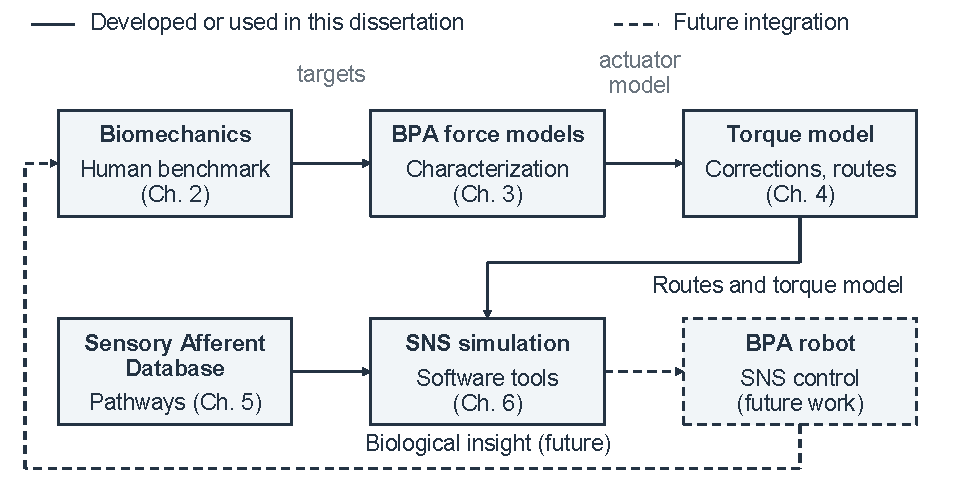
\includegraphics[width=\textwidth]{roadmap.pdf}
\caption[Dissertation roadmap]{The program's flow. The biomechanics benchmark of the background chapter feeds the actuator force characterization, whose correction factors and redesigned routes carry the models to the joint; the Sensory Afferent Database fixes the controller's sensory channels; and the simulation tools close the loop between converted body and synthetic nervous system. Solid blocks identify the models, evidence, and software developed or used in this dissertation. Dashed connections and the dashed robot block identify future integration and its intended return of biological insight to the benchmark.
}
\label{fig:roadmap}
\end{figure}

Appendix~\ref{app:muscle_calcs} documents the muscle force formulations and their cross-platform comparison, the BPA force model implementation, the muscle-path length and moment-arm calculations, and the compliance and wrapping-loss implementations. Appendix~\ref{app:neuron_equations} provides the neuron and synapse equations, spiking and non-spiking alike, used by the synthetic nervous system tools, relates those equations to their SNS-Toolbox implementation, and records the spiking-mirror calibration and the connectomes of the spinal-network models. Appendix~\ref{app:model_geometry} records the static BPA pathways, joint transformation matrices, bracket reference frames, stiffness and compliance parameters, adopted correction-term values, and the redesigned extensor route geometry.
